%
%  proposta
%
%  Created by Ricardo de Cillo on 2012-05-27.
%  Copyright (c) 2012 __MyCompanyName__. All rights reserved.
%
\documentclass[a4paper,11pt]{article}

% Use utf-8 encoding for foreign characters
\usepackage[brazil]{babel}
\usepackage[utf8]{inputenc}
\usepackage[T1]{fontenc}

% Setup for fullpage use
\usepackage{fullpage}

\usepackage{anysize}
\marginsize{2cm}{2cm}{1cm}{1cm}

% Uncomment some of the following if you use the features
%
% Running Headers and footers
%\usepackage{fancyhdr}

% Multipart figures
%\usepackage{subfigure}

% More symbols
%\usepackage{amsmath}
%\usepackage{amssymb}
%\usepackage{latexsym}

% Surround parts of graphics with box
\usepackage{boxedminipage}

% Package for including code in the document
\usepackage{listings}

% If you want to generate a toc for each chapter (use with book)
\usepackage{minitoc}

% This is now the recommended way for checking for PDFLaTeX:
\usepackage{ifpdf}

%\newif\ifpdf
%\ifx\pdfoutput\undefined
%\pdffalse % we are not running PDFLaTeX
%\else
%\pdfoutput=1 % we are running PDFLaTeX
%\pdftrue
%\fi

\ifpdf
\usepackage[pdftex]{graphicx}
\else
\usepackage{graphicx}
\fi


\title{Aplicação de análise morfológica para segmentação de páginas em imagens de documentos}
\author{ Aluno: Ricardo de Cillo \\ Supervisora: Nina S. T. Hirata }

\date{}

\begin{document}


\maketitle


\section{Objetivo}
	Uma das aplicações da teoria de visão computacional é a análise de imagens de documentos. O objetivo desta aplicação é extrair informações sobre o conteúdo e estrutura de um documento digitalizado. Uma das etapas envolvidas é a segmentação de página que consiste na identificação de áreas da imagem correspondentes à elementos estruturais, tais como títulos, legendas e blocos de texto. Neste trabalho iremos explorar métodos morfológicos aplicados à segmentação de páginas. A qualidade da solução obtida será medida e comparada, segundo os mesmo critérios aplicados à resultados considerados estado da arte por pesquisadores da área \cite{10.1109/ICDAR.2007.207}.

\section{Metodologia}

A análise de imagens de documentos, ou apenas análise de documentos, é um campo de pesquisa ativo apesar de ter sido bastante explorado nas últimas décadas. Isto se deve a sua importância prática e a complexidade dos problemas abordados. Delimitamos o escopo deste trabalho à análise de layout, como indicado no diagrama \ref{fig:context1} adaptado de \cite{Kasturi_OGorman_Govindaraju_2002}.

\begin{figure}[htb!]
\begin{center}
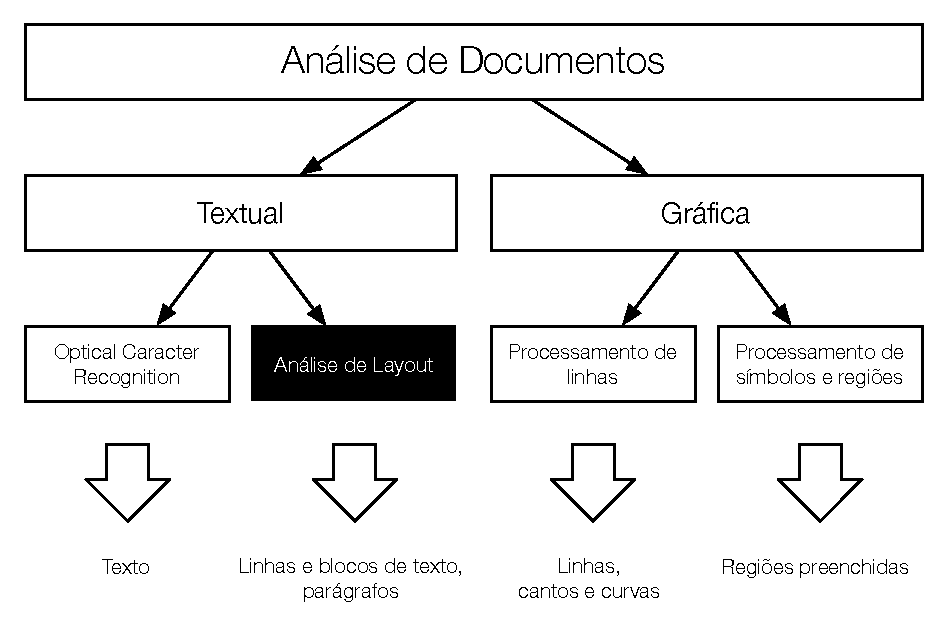
\includegraphics{assets/document_processing_areas_hierarquies.pdf}
\end{center}
\caption{Contextualização do tema do trabalho entre as áreas da análise de documentos.}
\label{fig:context1}
\end{figure}

Uma grande diversidade de métodos já foram explorados na solução deste problema. Em \cite{Antonacopoulos95representationand} os autores propõem um método que observa a distribuição dos espaços em branco em um documento para classificar a região em texto ou não. Já em \cite{Moll07documentcontent} extrai-se características dos pixels e sua vizinhança, classificando-os e depois agrupando-os em regiões.

Neste trabalho utilizaremos operadores morfológicos \cite{Serra:1983:IAM:1098652}, uma ferramenta clássica na área de visão computacional, para segmentar a imagem. A construção de operadores morfológicos complexos a partir da combinação de operadores simples pode ser uma tarefa difícil e demandar muita experiência. Portanto construiremos tais operadores de forma automática a partir de imagens de treinamento, como descrito em \cite{Tomita:1996:PrAuMa}.

\begin{figure}[htb!]
\begin{center}
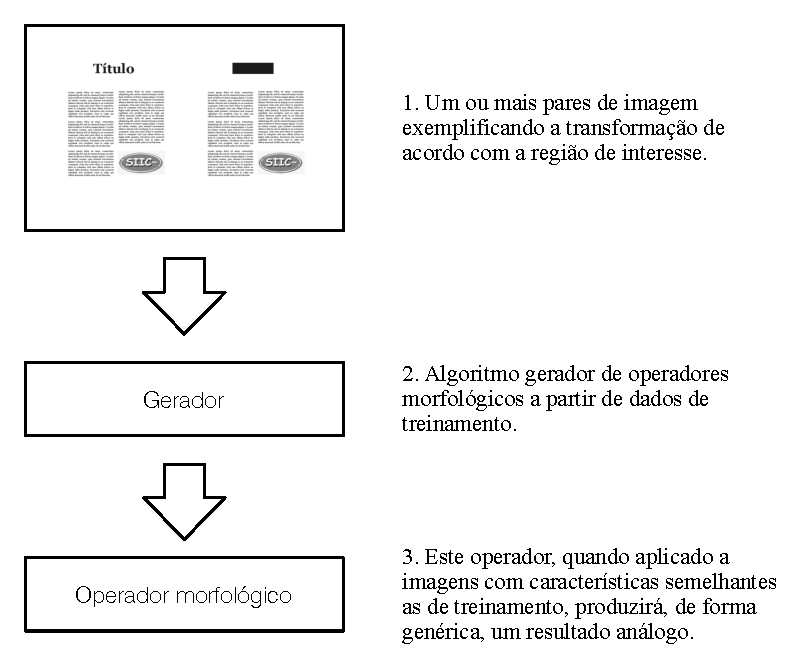
\includegraphics{assets/methodology.pdf}
\end{center}
\caption{Visão global do funcionamento.}
\label{fig:schema_overview}
\end{figure}

\bibliographystyle{plain}	% (uses file "plain.bst")
\bibliography{myrefs}		% expects file "myrefs.bib"

\end{document}
